
%Fichier: cours-html.tex
%Crée le 05 juil. 2008
%Dernière modification: 26 oct. 2019 22:31:42

\documentclass[10pt,dvipsnames, dvips, svgnames]{article}
%%%%%%%% mes package %%%%%%%%%%%%%%%%%
\usepackage[utf8]{inputenc}
\usepackage[T1]{fontenc}
\usepackage{lmodern}
\usepackage{tabularx}
\usepackage{enumerate}
\usepackage{multirow}
\usepackage{colortbl}%%%pour colorer les cases d'un tableau
\usepackage{amssymb}  %  pour  leqslant 
\usepackage[verbose,a4paper,tmargin=2.2cm,bmargin=1.5cm,lmargin=1.3cm,rmargin=1.3cm]{geometry} %%%%pour fixer les marges du texte
%mise en page
%\usepackage{lscape} %%% pour localement utiliser \begin{landscape}...\end{landscape}
\usepackage{multicol} %%%%
\usepackage{ulem}
\usepackage{array}
\usepackage[dvips,ps2pdf]{hyperref}
\usepackage{verbatim}
\usepackage{textcomp} %%%Pour autoriser les caractères ° etc...
\usepackage{amsfonts,t1enc} %%% pour avoir les ensembles N Z Q R C
\usepackage{amsmath}%%%pour dfrac  etc...
\usepackage{pstricks,pst-plot}
\usepackage{xcolor} % utiliser par exemple black!20
\usepackage[dvips,ps2pdf]{hyperref} %%%Pour les liens
\usepackage{graphicx} %%%%



\usepackage{fancyhdr,fancybox}  %%%%pour les hauts et bas de pages
\usepackage{graphicx} %%%%pour inclure les graphiques
\usepackage{lastpage} %%%%pour inclure le le nombre total de page
%\usepackage{makeidx}
\usepackage[Bjornstrup]{fncychap}
\usepackage{alltt}

%les fontes
%\usepackage{lmodern}
%\usepackage{frcursive} %pour la fonte cursuive
\usepackage{pifont} % pour la fonte ding
\usepackage{textcomp} %%%Pour autoriser les caractères ° etc...

\usepackage{pst-eucl} %%% pour les dessin geométrique pstricks %%%
\usepackage{multido}
\newcounter{numeroexo}[section]
\newcommand{\exerciceun}[1]{\par\stepcounter{numeroexo}\hspace{-0.5cm}\underline{\textbf{Exercice \arabic{numeroexo}}}\quad \textit{#1}\:}





% mon fichier listing se télécharge ic http://megamaths.free.fr/pdf/mes_listings.tex
\input{mes_listings.tex} %%% pour les listings R-cran xcas etc... %%%%

\usepackage[frenchb]{babel}
%%%%%%%%            %%%%%%%%%%%%%%%%%
\hypersetup{
     backref=true,    %permet d'ajouter des liens dans...
     pagebackref=true,%...les bibliographies
     hyperindex=true, %ajoute des liens dans les index.
     colorlinks=true, %colorise les liens
     breaklinks=true, %permet le retour à la ligne dans les liens trop longs
     urlcolor= blue, %couleur des hyperliens
     linkcolor= blue, %couleur des liens internes
     bookmarks=true, %créé des signets
     bookmarksopen=false,  %si les signets Acrobat sont créés,
                          %les afficher complètement.
     pdftitle={aide mémoire}, %informations apparaissant dans
     pdfauthor={Meilland jean claude},     %dans les informations du document
     pdfsubject={Correspondance algorithmique python}       %sous Acrobat.
}



%\renewcommand{\vec}[1]{\overrightarrow{#1}}%écriture d'un vecteur
%\newcommand{\cc}[1]{\mathcal{C} _{#1}}%pour écrire Cf la courbe représentative
%\newcommand{\dd}[1]{\mathcal{D} _{#1}}%pour écrire Df le domaine de définition
%\newcommand{\R}{\mathbb{R}}
%\newcommand{\N}{\mathbb{N}}
%\newcommand{\C}{\mathbb{C}}
%\newcommand{\e}{\mathrm{e}}
\newcommand{\code}[1]{\fcolorbox{black}{cyan!10}{\lstinline!#1!}}

\newcounter{Chapter}
\newcounter{Sec}[Chapter]
\newcounter{Subsec}[Sec]
%\newcounter{Subsubsection}[Subsec]


%\newsavebox\boxofgeogebra

%\newcommand{\Chapter}[1]{\pdfbookmark[1]{#1}{chapter\theChapter}\stepcounter{Chapter}\chead{\colorbox{black!15}{ \Large\textbf{\Roman{Chapter} #1}}  }}
\newcommand{\Chapter}[1]{\stepcounter{Chapter}\chead{\colorbox{black!15}{ \Large\textbf{\Roman{Chapter} #1}}  }}


\newlength\taille
\newenvironment{Sec}[1]
{
\stepcounter{Sec}
\taille=\linewidth\advance\taille by -0.4cm % On réduit la largeur du cadre gris
\pdfbookmark[2]{#1}{Sec\theChapter-\theSec}
\begin{center}
\colorbox{black!15}{
	\begin{minipage}{\taille}
	\begin{flushleft}
	\textbf{
		\arabic{Sec}  #1
	}
	\end{flushleft}
	\end{minipage}\par
}\end{center}
}

\newcommand{\Subsec}[1]{\stepcounter{Subsec} \underline{\textbf{\alph{Subsec}~ #1} } \\}

%\setcounter{secnumdepth}{1}% enlève la numérotation après les sections
\usepackage{titlesec}


%redéfinition des sections
\titleformat{\section}
   {\large\selectfont\bfseries}% apparence commune au titre et au numéro  %\normalfont\fontsize{11pt}{13pt}
   {\thesection}% apparence du numéro
   {1em}% espacement numéro/texte
   {}% apparence du titre
\titlespacing{\subsubsection}{1pt}{1pt}{1pt}  %\titlespacing{\section}{espace horizontal}{espace avant}{espace après}


%redéfinition des subsubsections
\titleformat{\subsubsection}[hang]
   {\selectfont\bfseries}% apparence commune au titre et au numéro  %\normalfont\fontsize{11pt}{13pt}
   {\alph{subsubsection}\string)\ }% apparence du numéro
   {2pt}% espacement numéro/texte
   {\underline}% apparence du titre
\titlespacing{\subsubsection}{2pt}{1pt}{2pt}  %\titlespacing{\section}{espace horizontal}{espace avant}{espace après}

%\setlength{\parindent}{0pt}
\pagestyle{fancy}  
\lhead{\small\textsc{Icn: Pablo neruda}}
\chead{\small\textsc{TP HTML}}
\rhead{Page \thepage/\pageref{LastPage} } \cfoot{}
\renewcommand{\headrulewidth}{1pt}
\renewcommand{\footrulewidth}{0pt}

% Pour les algorithmes


\usepackage[french,boxed,vlined]{algorithm2e}  %,linesnumbered,inoutnumbered
%SetKwData{fonction}{fonction: }
\SetKwInput{Fonction}{\textbf{fonction}}
\SetKwInput{Procedure}{\textbf{procédure} }
\SetKwInput{Variable}{\textbf{Variable}}
\SetKwInput{Constante}{\textbf{Constante}}
\SetKw{EntSor}{E/S}
\SetKw{Ent}{E}
\SetKw{Sor}{S}
%\SetKwInput{Variable}{Variable}
%\SetKw{fonction}{fonction:}
\SetKwSwitch{Selon}{Cas}{Autre}{selon}{}{cas où}{autres cas}{fin d'alternative}
\SetAlCapFnt{\color{red}}

%\setlength{\parskip}{2pt}
%Pour l'environnement multicolonne
%\setlength{\columnseprule}{0pt}
%\setlength{\columnsep}{0.5cm}

%\setlength{\parindent}{1cm} %
%\setlength{\parskip}{1cm plus4mm minus3mm}



%%%% debut macro figure à gauche \figgauche %%%%
 \newlength\jataille
 \newcommand{\figgauche}[3]%
 {\jataille=\linewidth\advance\jataille by -#1
 %\jataille=\textwidth\advance\jataille by -#1
 \advance\jataille by -1cm
 \begin{minipage}[t]{#1}
 #2
 \end{minipage}\hfill
 \begin{minipage}[t]{\jataille}
  #3
 \end{minipage}}
 %%%% fin macro %%%%

 %%%% debut macro figure à droite \figdroite%%%%
 \newlength\jatail
 \newcommand{\figdroite}[3]%
 {\jatail=\linewidth\advance\jatail by -#1
 \advance\jatail by -0.5cm
\begin{minipage}[t]{\jatail}
 #2
 \end{minipage}
 \hfill
\begin{minipage}[t]{#1}
  #3
\end{minipage}}

\setlength\parindent{0pt}%noident






\begin{document}


\section{Introduction au World Wide Web}
\subsection{L'Internet et le Web, quelle différence ?}


\textbf{Internet} est un réseau informatique mondial.

Le \textbf{World Wide Web}, que l'on appelle le plus souvent \textbf{Web}, est un des services disponibles sur Internet.

D'autres services disponibles sur Internet sont par exemple la messagerie électronique (\textbf{email}) ou le transfert de fichier (\textbf{FTP})

\subsubsection{Le Web ou World Wide Web, à quoi ça sert ?}

Le Web ("la toile" en français) est un système permettant de visualiser et d'échanger des informations à distance.

Les informations sont présentées sur des pages Web et reliées les unes aux autres par des liens hypertextes.
	
\subsubsection{Qu'est-ce qu'une page Web ? Qu'est-ce qu'un site Web ?}

Une page Web est généralement un fichier texte écrit dans un langage informatique baptisé HTML.\\
Ce fichier peut contenir des images ou d'autres contenus multimédias (audio, vidéo, application).

Un site Web est un ensemble de pages Web reliées les unes aux autres par des liens hypertextes et accessible en ligne à une adresse.


\subsubsection{Le langage HTML}

\textbf{HTML} est l'acronyme d'\textbf{H}yper\textbf{t}ext \textbf{M}arkup  \textbf{L}anguage qui peut se traduire ainsi : langage hypertexte à balise.

Le HTML est un langage informatique utilisant des \textbf{textes} et des \textbf{balises}. On peut utiliser un simple éditeur de texte pour créer un fichier HTML.


Pour visionner un fichier en HTML on utilise un navigateur. Un navigateur est un logiciel qui va lire le code HTML et l'interpréter. Chaque balise donne au navigateur des informations sur comment afficher tel ou tel élément.

\subsubsection{À propos des balises}

Une balise (markup en anglais) est un mot clé qui va donner des indications au navigateur sur ce qu'il doit afficher.

Une balise HTML commence par le caractère \og < \fg et termine par le caractère \og > \fg .

Les caractères qui ne sont pas compris entre les signes \og < \fg et \og > \fg sont donc considérés comme du texte et seront affichés tel quel par le navigateur.


\begin{list}{$\bullet$}{}
	\item  Il existes des balises ouvrantes et des balises fermantes qui correspondent au début et la fin d'une instruction.
	\item Les balises de fermeture sont identiques à celles d'ouverture à l'exception de l'ajout d'un caractère \og / \fg (slash) pour signaler la fermeture. Ce caractère se place juste après le signe \og > \fg (inférieur)
	\end{list}

\subsubsection{Structure d'un fichier HTML}

Un fichier HTML (un document HTML) commence par l'ouverture d'une balise <html> et se termine par la balise fermante </html> 

Tous les fichiers HTML sont composés d'une entête (balise "head") et d'un corps (balise "body"). L'entête contient des informations sur la page.\\
Le corps contient le contenu de la page.

\lstset{title={},caption={Exemple}, language=html}
\begin{lstlisting}
<html>
  <head>
  </head>
  <body>
    Texte de la page ici.
  </body>
</html>
\end{lstlisting}


\subsubsection{Principe du Web}

Structure simplifiée d’une adresse, d’une URL :

protocole :// serveur/ressource


\url{http://www.univ-nancy2.fr/formations/calendrier_licence.html}

protocole: Hyper Text Transfer\\
nom du serveur : nom de domaine de l'ordinateur hébergeant la ressource demandée:  \\
Emplacement de la ressource sur le serveur:  en général emplacement (répertoire) et nom du fichier demandé (html ou autre).



%Souvent .htm, html. Mais également .asp,php... pour des pages générées dynamiquement.

\newpage
\subsubsection{HTTP et HTML}

\begin{list}{$\bullet$}{}
\item HTTP=Hypertext Transfer Protocol :
	\begin{list}{-}{}
	\item Protocole utilisé pour transférer des fichiers (html, mais pas forcément) entre un serveur http et un navigateur
	\end{list}
\item Que se passe-t-il lorsque je consulte une page web ?
	\begin{list}{-}{}
	\item Grâce à l’url de la page, mon navigateur consulte un DNS (qui peut lui-même demander à un autre DNS) le serveur qui l’héberge,
	\item Mon navigateur demande au serveur (grâce à HTTP) la page 
	\item Le serveur la renvoie (toujours grâce à HTTP)
	\item Mon navigateur affiche la page (grâce à HTML)
	\end{list}
\item HTML=Hypertext Markup Language :
	\begin{list}{-}{}
	\item Langage de balisage hypertexte
	\item Langage informatique créé pour écrire des pages web
	\item Cours détaillés sur html dans une prochaine séance
	\end{list}
\end{list}



\begin{lstlisting}
<!DOCTYPE html>
<html>
<head>
  <!-- En-tête de la page -->
  <meta charset="utf-8" />
  <title>Titre</title>
</head>
<body>
  <!-- Corps de la page -->
</body>
</html>
\end{lstlisting}
\newpage


\section{HTML}

\begin{list}{$\bullet$}{}
\item \url{https://www.pierre-giraud.com/html-css/cours-complet/cours-html-css-presentation.php}
\end{list}

\subsection{Préparation}


%HTML n'est pas un langage de programmation (comme le JavaScript par exemple), ici, pas question de conditions, de boucles....c'est un langage de description.

\textbf{HTML} est l'abréviation de \textbf{HyperText Markup Language}, soit en français \og  langage de balisage hypertexte \fg.

Ce langage a été créé en 1991 et a pour fonction de structurer et de donner du sens à du contenu.

Grâce au HTML, on va par exemple pouvoir indiquer au navigateur que tel texte doit être considéré comme un simple paragraphe ou que tel autre est un titre.

Pour écrire les fichiers html on a deux solutions.

\begin{enumerate}
\item Écrire directement le code avec un éditeur de texte (Attention à ne pas confondre avec un traitement de texte comme openoffice, word \ldots).\\
	\begin{list}{\ding{212}}{}
	\item Lancer  \textbf{\textit{notepad++}} ou  \textit{\textbf{pyzo}}.  
	%	Au lycée on peut utiliser \textbf{\textit{notepad++}} \textit{\textbf{pyzo}}  pour écrire directement le code puis de l'ouvrir avec un navigateur.\\
	\item Écrire le code  suivant:\\
\lstset{title={},caption={}, numbers=left, firstnumber=1, language=html}
\begin{lstlisting}
<!DOCTYPE html>
<html>
<head>
  <!-- En-tête de la page -->
  <title>Titre</title>
  <meta charset="utf-8" />
</head>
<body>
  <!-- Corps de la page -->
  <p>Hello</p>
</body>
</html>
\end{lstlisting}
\item Enregistrer le fichier dans votre session,  ouvrez un navigateur de votre choix (Firefox, chrome \dots), et ouvrez le fichier.
\end{list}
\item Utiliser un  éditeur en ligne.  Nous utiliserons le site \href{https://jsfiddle.net/}{jsfiddle.net}. %(pour python c'est \url{https://repl.it/repls})
	\begin{list}{\ding{212}}{}
\item Lancer le navigateur de votre choix (Firefox ou chrome), taper \url{http://jsfiddle.net/} dans la barre d'adresse.\\
Vous devriez voir apparaître ceci :
\begin{center}
\includegraphics[width=14cm]{images/jsfile1}
\end{center}
Si vous avez déjà du texte alors cliquez sur\raisebox{-0.1cm}{\includegraphics[width=0.6cm]{images/icone-jsfile}}\ding{212} Empty 
\item  Recopier le texte écrit entre les balises \textbf{\textit{<body>}} dans la section \textbf{HTML}
\lstset{title={},caption={}, numbers=left, firstnumber=1, language=html}
\begin{lstlisting}
  <!-- Corps de la page -->
  <p>Hello</p>
\end{lstlisting}
\item Pour visualiser cliquez  sur l'icone \textit{\textbf{Run}}. 
\end{list}
\end{enumerate}


À noter :\begin{list}{-}{}
\item  La ligne numéro 6 sert pour préciser  l'encodage utf8 (ainsi les accents \og français \fg sont  bien pris en compte).\\
Pour HTML5 l'encodage par défaut des caractères est UTF-8 .
\item  Lorsque vous réaliserez une nouvelle page html, vous ferez un \og copier-coller \fg de cet en-tête.
\item Tous les documents html que vous enregistrerez devront avoir l'extension : \textbf{.html}
\end{list}


\subsection{Organiser une page :}

\subsubsection{Les balises}

Les pages HTML sont remplies de ce qu'on appelle des \textbf{balises}. Celles-ci sont invisibles à l'écran pour vos visiteurs, mais elles permettent à l'ordinateur de comprendre ce qu'il doit afficher.\\
Les balises se repèrent facilement. Elles sont entourées de \og \textbf{chevrons} \fg, c'est-à-dire des symboles < et > ,comme ceci :  \textcolor{Blue}{< balise >}. Elles indiquent la nature du texte qu'elles encadrent (un titre, une image \dots).\\ %Elles veulent dire par exemple \og Ceci est le titre de la page \fg, \og Ceci est une image \fg, \og Ceci est un paragraphe de texte \fg \dots\\
On distingue deux types de balises : les \textbf{balises en paires} et les \textbf{balises orphelines.}

\begin{list}{$\bullet$}{}
\item Les balises en paires s'ouvrent, contiennent du texte, et se ferment plus loin.\\
	Voici à quoi elles ressemblent :  \textcolor{Blue}{< title > Ceci est un titre < /title >}.
\item Les balisent orphelines servent souvent à insérer un élément à un endroit précis, par exemple une image.\\
Voici à quoi elles ressemblent  \textcolor{Blue}{<image />}.
\end{list}

%\subsubsection{Les incontournables}
\subsubsection{Base d'une page html}
\begin{list}{$\bullet$}{}
\item   \textcolor{Blue}{< ! DOCTYPE html >} signifie que la page est écrite en \textbf{HTML5}
\item   \textcolor{Blue}{<html> \dots </html>} englobe tout le contenu de la page
\item   \textcolor{Blue}{<head> \dots </head>}: (header) fournit des informations générales (métadonnées) sur le document, incluant son titre et des liens vers des scripts et feuilles de style. \\
\lstset{title={},caption={}, numbers=left, firstnumber=3,language=html}
\begin{lstlisting}
<head>
  <!-- En-tête de la page -->
  <title>Titre</title>
  <meta charset="utf-8" />
</head>
\end{lstlisting}
	Cette balise encadre des informations générales sur la page comme le titre, l'encodage (gestion des caractères spéciaux comme les accents en français.\\
Enlever la ligne 6 pour voir ce que ça donne.
\item   \textcolor{Blue}{<body> \dots </body>} encadrent le contenu du site web.
\end{list}

\subsection{ Organiser son texte}
\subsubsection{Les paragraphes}

\begin{list}{$\bullet$}{}
\item \textcolor{Blue}{<p> \dots </p>} pour encadrer un paragraphe
\item \textcolor{Blue}{<br />} pour sauter une ligne
\end{list}
%\colorbox{SteelBlue}{\textcolor{white}{Écrire quelques lignes sur votre page et tester le résultat.}}

\hypersetup{urlcolor=white}
\colorbox{SteelBlue}{\textcolor{white}{Écrire quelques lignes utilisant ces balises  sur \href{https://jsfiddle.net/}{jsfiddle.net}}}
\hypersetup{urlcolor=blue}


\subsubsection{Les titres}

En HTML, on peut utiliser six niveaux de titres différents.  On a donc six balises de titres différentes :

\begin{list}{$\bullet$}{}
\item  \textcolor{Blue}{<h1> \dots </h1>} : signifie \og titre très important \fg.
\item  \textcolor{Blue}{<h2> \dots </h2>} : signifie \og titre important \fg.
\item  \textcolor{Blue}{<h3> \dots </h3>} : pareil, c'est un titre un peu moins important.
\item  \textcolor{Blue}{<h4> \dots </h4>} : titre encore moins important.
\item  \textcolor{Blue}{<h5> \dots </h5>} : titre pas important.
\item  \textcolor{Blue}{<h6> \dots </h6>} : titre pas important du tout.
\end{list}


\hypersetup{urlcolor=white}
\colorbox{SteelBlue}{\textcolor{white}{Écrire quelques lignes   utilisant ces balises  sur \href{https://jsfiddle.net/}{jsfiddle.net}}}
\hypersetup{urlcolor=blue}

\subsubsection{Les listes}

Les listes nous permettent souvent de mieux structurer notre texte et d'ordonner nos informations.\\
Il existe plusieurs types de listes dont :


\begin{list}{$\bullet$}{}
\item  les listes à puces (\textbf{unordonned} en anglais) : \textcolor{Blue}{<ul> \dots </ul>}.
\item  les listes numérotées (\textbf{ordonned} en anglais) : \textcolor{Blue}{ <ol> \dots </ol>}.
Dans les deux cas, les différentes lignes sont encadrées par les balises  \textcolor{Blue}{<li> \dots </li>}.
\end{list}

Exemples :


\begin{minipage}[t]{0.5\linewidth}
\lstset{title={},caption={}, language=html}
\begin{lstlisting}
<ul>
  <li> Fraises </li>
  <li> Framboises </li>
  <li> Cerises </li>
</ul>
\end{lstlisting}
\end{minipage}
\begin{minipage}[t]{0.5\linewidth}
\lstset{title={},caption={}, language=html}
\begin{lstlisting}
<ol>
  <li> Fraises </li>
  <li> Framboises </li>
  <li> Cerises </li>
</ol>
\end{lstlisting}
\end{minipage}

\hypersetup{urlcolor=white}
\colorbox{SteelBlue}{\textcolor{white}{Tester ces lignes de code sur \href{https://jsfiddle.net/}{jsfiddle.net}.}}
\hypersetup{urlcolor=blue}

%\begin{minipage}[t]{0.5\linewidth}
%\begin{list}{$\bullet$}{}
%\item Fraises 
%\item Framboises
%\item Cerises 
%\end{list}
%\end{minipage}
%\begin{minipage}[t]{0.5\linewidth}
%\begin{enumerate}
%\item Fraises
%\item Framboises
%\item Cerises
%\end{enumerate}
%\end{minipage}



\subsubsection{Les tableaux}

Pour créer un tableau simple, nous allons avoir besoin de trois éléments HTML :

\begin{list}{$\bullet$}{}
\item La balise \textbf{\textit{<table>}} ( \og  tableau \fg en français) va définir le tableau;
\item     La balise \textbf{\textit{<tr>}}, pour \og   table row \fg  va nous servir à introduire une nouvelle ligne;
\item     La balise \textbf{\textit{<td>}}, pour \og table data \fg ou \og  donnée de tableau  \fg en français va nous permettre d'ajouter des cellules.
\item La balise \textbf{\textit{<th>}} pour \og   table header \fg  est utilisé pour définir les titres d'un tableau html. %Elle  est équivalente à la balise \textbf{\textit{<td>}} en terme de propriétés.
\end{list}

Exemples :

\begin{minipage}[t]{0.6\linewidth}
\lstset{title={},caption={}, language=html}
\begin{lstlisting}
<table>
  <tr><th>Nom</th><th>prénom</th><th>âge</th></tr>
  <tr><td>Onette</td><td>Camille</td><td>15</td></tr>
  <tr><td>Vanille</td><td>Douglas</td><td>16</td></tr>
  <tr><td>Bijoba</td><td>Joe</td><td>16</td></tr>
</table>
\end{lstlisting}
\end{minipage}
\begin{minipage}[t]{0.4\linewidth}
\vspace{1cm}
\begin{center}
%\raisebox{-2cm}{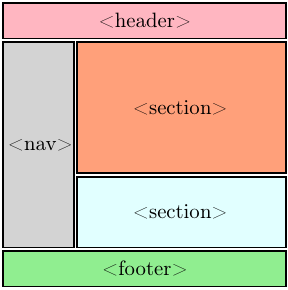
\includegraphics[width=3cm]{images/html1}}
\hypersetup{urlcolor=white}
\colorbox{SteelBlue}{\textcolor{white}{Tester ces lignes de code sur \href{https://jsfiddle.net/}{jsfiddle.net}}}
\hypersetup{urlcolor=blue}
\end{center}
\end{minipage}

Pour obtenir les lignes il faut utiliser du code \textbf{\textit{CSS}} que nous verrons donc  plus tard.


\begin{list}{$\bullet$}{}
\item \textbf{\textit{colspan}} Spécifie le nombre de colonnes sur lequel s'étendra la cellule.  Cela permet de scinder les colonnes.
\item \textbf{\textit{rowspan}} spécifie le nombre de lignes sur lequel s'étendra la cellule. Cela permet de scinder les lignes.
\end{list}

Exemple:

%\begin{minipage}[t]{0.82\linewidth}
\begin{minipage}[t]{\linewidth}
\lstset{title={},caption={}, language=html}
\begin{lstlisting}
<table cellpadding="3px" cellspacing="0px" rules="all" style="border:solid 1px black;
border-collapse:collapse;  text-align:center;"> 
   <tr>  <th>Titre 1</th> <th>Titre 2</th> </tr> 
   <tr>  <td>Valeur1</td> <td>Valeur2</td> </tr> 
   <tr> 
      <td colspan="2"  style="background-color:lightyellow;">Cellule avec colspan</td> 
   </tr> 
   <tr> 
      <td rowspan="2" style="background-color:lightsteelblue;">Cellule avec rowspan</td> 
      <td>Valeur 3</td> 
   </tr> 
   <tr>       <td>Valeur 4</td>    </tr> 
</table> 
\end{lstlisting}
\end{minipage}
%\begin{minipage}[t]{0.18\linewidth}
%\begin{center}
%\raisebox{-5cm}{\includegraphics[width=3cm]{images/html2}}
%\scriptsize
%\setlength{\tabcolsep}{0.05cm}
%\begin{tabular}[]{|c |c |}
%	\hline \textbf{Titre 1} & \textbf{Titre 2} \\
%	\hline Valeur 1 & Valeur 2 \\
%	\hline \multicolumn{2}{|c|}{\cellcolor{LightYellow} Cellule avec colspan} \\
%	\hline \cellcolor{LightSteelBlue} & Valeur 3 \\
%	 \multirow{-2}{*}{\cellcolor{LightSteelBlue} Cellule avec rowspan}  & Valeur 4 \\
%	\hline 
%\end{tabular} 
%\normalsize
%\end{center}
%\end{minipage}

\hypersetup{urlcolor=white}
\colorbox{SteelBlue}{\textcolor{white}{Tester ces lignes de code sur \href{https://jsfiddle.net/}{jsfiddle.net}}}
\hypersetup{urlcolor=blue}

\subsubsection{Insérer des images}

%On utilise plusieurs type d'image:
%
%\begin{list}{$\bullet$}{}
%\item Le format \textbf{JPEG} (pour Joint Photographic Expert Group), ou plus communément \textbf{JPG} est un format qui permet généralement de compresser le poids d'une image par dix tout en conservant une très bonne qualité.
%\item Le \textbf{PNG} (Portable Network Graphic) est un format qui a été créé à l'origine pour remplacer le format GIF. Le grand intérêt de ce format est qu'il gère la transparence. Celui-ci a un très bon taux de compression tout en conservant une bonne qualité d'image.
%%\item  Le \textbf{SVG} ( \textit{Scalable Vector Graphics} ou  \textit{graphique vectoriel adaptable} en français) qui est un format vectorielle. Les navigateurs récents supportent ce format.
%\end{list}

L'insertion d'images  va se faire au moyen de la balise orpheline \textbf{\textit{<img  \dots />}} 

\begin{list}{$\bullet$}{}
\item L'attribut \textbf{\textit{src}} (pour source) va prendre comme valeur l'adresse de l'image (adresse relative ou absolue)
\item L'attribut \textbf{\textit{alt}} (pour alternative) va contenir un texte alternatif décrivant l'image. Ce texte va être affiché si l'image ne peut pas l'être pour une raison ou pour une autre, et est également très utile pour les non-voyants.
\item L'attribut \textbf{\textit{width}}  permet de fixer une taille précise.% (on peut aussi le faire avec css).
\end{list}

Exemple:

\begin{lstlisting}
<img alt='Pablo Neruda' src='https://upload.wikimedia.org/wikipedia/commons/8/86/Pablo_Neruda_1963.jpg' width=200px />
\end{lstlisting}



\hypersetup{urlcolor=white}
\colorbox{SteelBlue}{\textcolor{white}{Tester ces lignes de code sur \href{https://jsfiddle.net/}{jsfiddle.net}.}}
\hypersetup{urlcolor=blue}


\subsubsection{Les liens}

\textbf{\textit{Html}} (Hyper Text Markup Language) est un langage hypertexte  qui vous permet en cliquant sur un mot, généralement souligné (ou une image) de vous transporter;

%\begin{list}{$\bullet$}{}
%\item  vers un autre endroit du document. 
%\item  vers un autre fichier Html situé sur votre ordinateur. 
%\item  vers un autre ordinateur situé sur le Web. 
%\end{list}

%Ce système d'hypertexte vous est familier car se sont ces liens qui vous permettent de surfer de page en page et qui constituent l'essence du Web et des documents Html.

\begin{list}{\ding{212}}{}
\item Les \textbf{liens externes}.

Les liens externes sont des liens ramenant vers des pages d'autres sites.


\begin{lstlisting}
<h1>Les liens</h1>
<p>Cliquez sur <a href="http://wikipedia.org">ce lien </a>pour aller sur Wikipédia.</p>
\end{lstlisting}


\hypersetup{urlcolor=white}
\colorbox{SteelBlue}{\textcolor{white}{Tester ces lignes de code sur \href{https://jsfiddle.net/}{jsfiddle.net}.}}
\hypersetup{urlcolor=blue}

\item Les \textbf{liens internes} en HTML

Les liens internes vont être des liens ramenant vers d'autres pages au sein d'un même site.

Dans ce cas, nous allons renseigner une \textbf{valeur relative} pour notre attribut \textit{href}.

Créez les fichiers suivants:

\lstset{title={},caption={\textbf{test-lien1.html}}, numbers=left, firstnumber=1, language=html}
\begin{lstlisting}
<!DOCTYPE html>
<html>
<head>
  <title>Les liens en HTML</title>
  <meta charset="utf-8" />
</head>
<body>
<h1>Les liens</h1>
<p>Page de départ</p>
<p>Cliquez pour accéder à <a href="test-lien2.html">la deuxième page</a>.</p>
<body>
</html>
\end{lstlisting}

\lstset{title={},caption={\textbf{test-lien2.html}}, language=html}
\begin{lstlisting}
<!DOCTYPE html>
<html>
<head>
  <title>Les liens en HTML</title>
  <meta charset="utf-8" />
</head>
<body>
<p>Deuxièmes page</p>
<body>
</html>
\end{lstlisting}

\hypersetup{urlcolor=white}
\colorbox{SteelBlue}{\textcolor{white}{Ouvrez un navigateur puis ouvrir la page test-lien1.html}}
\hypersetup{urlcolor=blue}

\end{list}


\subsection{Un peu de mise en forme}

Tout document \textit{Html} contient en majorité du texte. Voici comment l'agrémenter par quelques balises élémentaires.


\begin{list}{$\bullet$}{}
\item   \textcolor{Blue}{<!-- \dots -->}: Pour écrire un commentaire. Le texte n'est pas affiché.
\item   \textcolor{Blue}{<b> \dots </b>}: pour mettre le texte en   Gras (Bold en anglais).
\item   \textcolor{Blue}{<strong> \dots </strong>}: indique que le texte a une importance particulière (\textit{bold}).
\item   \textcolor{Blue}{<i> \dots </i>}:   pour mettre le texte en   \textit{Italique}.
\item   \textcolor{Blue}{<em> \dots </em>}:  est utilisé afin de marquer un texte sur lequel on veut insister (\textit{Italic}).
\item   \textcolor{Blue}{<mark> \dots </mark>}: représente un texte marqué  à cause de sa pertinence dans le contexte. \\
Il peut par exemple être utilisé afin d'indiquer les correspondances d'un mot-clé recherché au sein d'un document.
\item   \textcolor{Blue}{<center> \dots </center>}: pour centrer du texte.
%\item   \textcolor{Blue}{<> \dots </>}:
%\item   \textcolor{Blue}{<<++>> \dots </<++>>}:
\end{list}

%\begin{tabular}[]{|c |c | >{\centering}m{4cm}| >{\centering}m{6cm} |}
%\hline Gras &  [Bold] & <b>\dots</b>\\ <strong> \dots </strong> & Début et fin d'une zone en gras \tabularnewline
%\hline Italique & [Italic] & <i>\dots</i>\\<em> \dots </em> & Début et fin d'une zone en italique \tabularnewline
%\hline À la ligne & [Line break] & <br /> & Aller à la ligne\tabularnewline
%\hline Commentaires & [Comments] & <!-- commentaire  --> &  Ne pas afficher \tabularnewline
%\hline  Centrage  & [Center] & <center> \dots </center> & Centrer\tabularnewline
%\hline 
%\hline 
%\end{tabular} 

\subsection{Structurer sa page}

En général, une page web est constituée d'un en-tête (tout en haut), de menus de navigation (en haut ou sur les côtés), de différentes sections au centre… et d'un pied de page (tout en bas).


\figdroite{5cm}
{
HTML5 a introduit des balises permettant de structurer ses pages.

\begin{list}{$\bullet$}{}
\item   \textcolor{Blue}{<header> \dots </header>}: l'en-tête pour  le logo, la  bannière de notre site  \dots
\item   \textcolor{Blue}{<footer> \dots </footer>}: le pied de page.
\item   \textcolor{Blue}{<nav> \dots </nav>}: principaux liens de navigation ou le menu.
\item   \textcolor{Blue}{<section> \dots </section>}: permet de créer des sections de page
%\item   \textcolor{Blue}{<aside> \dots </aside>}: pour les informations complémentaires
%\item   \textcolor{Blue}{<article> \dots </article>}: pour un  article indépendant (ou  autonome de la page), c'est à dire une partie de la page qui pourrait ainsi être reprise sur un autre site.
\end{list}
}{\vspace{-0.4cm}
\psset{xunit=0.6cm , yunit=0.5cm}
\begin{center}
\begin{pspicture*}[shift=-4cm](-.1,-.1)(8.1,8.1)
\psframe[fillstyle=solid,fillcolor=LightGreen](0,0)(8,1)%footer
\psframe[fillstyle=solid,fillcolor=LightCyan](2.1,1.1)(8,3.1)%section2
\psframe[fillstyle=solid,fillcolor=LightSalmon](2.1,3.2)(8,6.9)%section1
\psframe[fillstyle=solid,fillcolor=LightGray](0,1.1)(2,6.9)%nav
\psframe[fillstyle=solid,fillcolor=LightPink](0,8)(8,7)%header
\rput(4,0.5){<footer>}
\rput(4,7.5){<header>}
\rput(5,5.05){<section>}
\rput(5,2.1){<section>}
\rput(1.05,4){<nav>}
\end{pspicture*}
\end{center}
}

\vspace{-0.8cm}


\subsection{TP}

Je désire avoir un livre de cuisine avec quatre recettes de cuisine (une entrée, un plats et deux desserts) que vous aimez bien.

Chaque recettes doit contenir la liste des ingrédients, une image du plat et le texte de la recette.

Le fichier \textbf{\textit{Recettes.html}} doit contenir:

\begin{list}{$\bullet$}{}
\item Première partie : Les entrée
\item Deuxième  partie:  Les plats
\item Troisième partie : Les desserts.
\end{list}

Me faire vérifier puis après transformer ce site en 4 pages.

\begin{list}{$\bullet$}{}
\item Un page \textbf{\textit{Recettes.html}} avec des liens vers les recettes
\item Une page \textbf{\textit{entree.html}} avec les recettes des entrées.
\item Une page \textbf{\textit{plat.html}}avec les recettes des plats.
\item Une page \textbf{\textit{dessert.html}} avec les recettes des desserts.
\end{list}


\section{CSS}

\subsection{Préparation}



\textbf{CSS} est le diminutif de \textbf{Cascading StyleSheets}, ou feuilles de styles en cascade.

Le CSS a été créé en 1996 et a pour rôle de mettre en forme du contenu en lui appliquant ce qu'on appelle des styles.

Le CSS va nous permettre par exemple de définir la taille, la couleur ou l'alignement d'un texte.

Nous allons donc utiliser le CSS sur notre code HTML, afin d'enjoliver le résultat visuel final.


Pour écrire le  code css on a deux solutions.

\begin{list}{\ding{212}}{}
\item Si on utilise \href{https://jsfiddle.net/}{jsfiddle.net} on écrit directement le code dans la partie \textbf{CSS}\\
\lstset{title={},caption={HTML}, language=HTML}
\begin{lstlisting}
<p>Voici un exemple</p>
\end{lstlisting}
	
\lstset{title={},caption={CSS}, language=css}
\begin{lstlisting}
p {
	color: red;
}
\end{lstlisting}
\item Si on écrit les page dans un fichier \textbf{\textit{HTML}} on peux écrire le code \textbf{\textit{css}} dans la même page mais il est préférable d'écrire le code \textbf{\textit{css}} dans un deuxième fichier avec l'extension \textbf{\textit{css}}. 

	Écrire le fichier \textbf{\textit{test-css.html}} avec le code suivant:
\lstset{title={},caption={test-css.html}, numbers=left, firstnumber=1, language=html}
\begin{lstlisting}
<!DOCTYPE html>
<html>
<head>
  <title>Exemple css</title>
  <meta charset="utf-8" />
  <link rel="stylesheet" href="monstyle.css" />
</head>
<body>
  <p>Hello</p>
</body>
</html>
\end{lstlisting}
\lstset{title={},caption={\textbf{\textit{monstyle.css}}}, numbers=left, firstnumber=1, language=css}
\begin{lstlisting}
p {
	color: red;
}
\end{lstlisting}

Ouvrez le fichier  \textbf{\textit{test-css.html}} avec un navigateur.


\end{list}




\subsection{Le principe}

\subsubsection{Par sélecteur de balise}

\colorbox{SteelBlue}{\textcolor{white}{Tester Les lignes de code ci-dessous sur \href{https://jsfiddle.net/}{https://jsfiddle.net}.}}

\lstset{title={},caption={}, language=html}
\begin{lstlisting}
<h1>titre 1</h1>
<p>ligne 1</p>
<p>ligne 2</p>
<p>ligne 3</p>
<h1>titre 2</h1>
<p>ligne 4</p>
<p>ligne 5</p>
\end{lstlisting}

\colorbox{SteelBlue}{\textcolor{white}{Regardez le résultat}} puis dans la partie \textbf{\textit{css}} écrire:

\lstset{title={},caption={}, language=css}
\begin{lstlisting}
p {
	color : red;
}
\end{lstlisting}

\colorbox{SteelBlue}{\textcolor{white}{Regardez le résultat.}}


\lstset{title={},caption={}, language=css}
\begin{lstlisting}
p h1 {
	color : red;
}
\end{lstlisting}

\colorbox{SteelBlue}{\textcolor{white}{Regardez le résultat.}}

\subsubsection{Par sélecteur d'\textbf{\textit{identités (id)}}}

Le sélecteur \string#\textbf{\textit{id}} nous permet de cibler un élément en particulier   plutôt qu'un type d'élément.\\
Une \textbf{\textit{id}} doit être \textbf{unique}.\\
Pour cibler un élément possédant un attribut \textbf{\textit{id}}, en CSS, il faudra préciser la valeur de l'attribut précédée d'un dièse (\string#).


\lstset{title={},caption={}, language=html}
\begin{lstlisting}
<h1>titre 1</h1>
<p id='rouge'>ligne 1</p>
<p id='bleu'>ligne 2</p>
<p>ligne 3</p>
<h1>titre 2</h1>
<p>ligne 4</p>
<p>ligne 5</p>
\end{lstlisting}

\lstset{title={},caption={}, language=css}
\begin{lstlisting}
#rouge {
	color : red;
}
#blue {
	color : blue;
}
\end{lstlisting}

\colorbox{SteelBlue}{\textcolor{white}{Regardez le résultat.}}



\subsubsection{Par sélecteur de \textbf{\textit{Classes}}.}

 Le sélecteur \textbf{\textit{.class}} nous permet de cibler un ensemble d'éléments possédant les mêmes propriétés.

 Pour cibler un élément possédant un attribut \textbf{\textit{class}}, en revanche, il faudra en CSS préciser la valeur de l'attribut précédée d'un point (\textbf{\textit{.}}).


\lstset{title={},caption={}, language=html}
\begin{lstlisting}
<h1>titre 1</h1>
<p class='rouge'>ligne 1</p>
<p class='bleu'>ligne 2</p>
<p>ligne 3</p>
<h1 class='rouge'>titre 2</h1>
<p class='rouge'>ligne 4</p>
<p class='bleu'>ligne 5</p>
\end{lstlisting}

\lstset{title={},caption={}, language=css}
\begin{lstlisting}
.rouge {
	color : red;
}
.blue {
	color : blue;
}
\end{lstlisting}

\colorbox{SteelBlue}{\textcolor{white}{Regardez le résultat}} puis modifier par:

\lstset{title={},caption={}, language=css}
\begin{lstlisting}
.rouge p{
	color : red;
}
.blue {
	color : blue;
}
\end{lstlisting}

\colorbox{SteelBlue}{\textcolor{white}{Regardez le résultat.}}


Il y a de nombreuses propriétés en \textbf{\textit{CSS}}.  Voici plusieurs liens intéressants.

\begin{list}{$\bullet$}{}
\item \href{https://www.cssdebutant.com/debuter-en-css-les-definitions-css.html}{Les propriétés CSS les plus utilisées sur \textit{cssdebutant.com}}
\item \href{https://openclassrooms.com/fr/courses/1603881-apprenez-a-creer-votre-site-web-avec-html5-et-css3/1608902-memento-des-proprietes-css}{Mémento des propriétés CSS sur \textit{openclassrooms}}
\item \href{http://www.css-faciles.com/proprietes-css-liste-alphabetique.php}{Toutes les propriétés CSS sur \textit{css-faciles.com}}
\end{list}



\section{Résumé  html}

Le \textbf{World Wide Web}, que l'on appelle le plus souvent \textbf{Web}, est un des services disponibles sur Internet.

D'autres services disponibles sur Internet sont par exemple la messagerie électronique (\textbf{email}) ou le transfert de fichier (\textbf{FTP})

\begin{list}{$\bullet$}{}
\item 
\lstset{title={},caption={Structure  générale}, language=html}
\begin{lstlisting}
<!DOCTYPE html>
<html>
<head>
  <!-- En-tête de la page -->
  <meta charset="utf-8" />
  <title>Titre</title>
</head>
<body>
  <!-- Corps de la page -->
</body>
</html>
\end{lstlisting}
\item \textcolor{Blue}{<p> \dots </p>} pour encadrer un paragraphe
\item \textcolor{Blue}{<br />} pour sauter une ligne
\item  \textcolor{Blue}{<h1> \dots </h1>} : signifie \og titre très important \fg.
\item  \textcolor{Blue}{<h2> \dots </h2>} : signifie \og titre important \fg.
\item  \textcolor{Blue}{<h3> \dots </h3>} : pareil, c'est un titre un peu moins important.  etc\dots
\item \begin{minipage}[t]{0.5\linewidth}
\lstset{title={},caption={Listes à puces (\textit{unordonned})}, language=html}
\begin{lstlisting}
<ul>
  <li> Fraises </li>
  <li> Framboises </li>
  <li> Cerises </li>
</ul>
\end{lstlisting}
\end{minipage}
\begin{minipage}[t]{0.5\linewidth}
\lstset{title={},caption={Listes numérotés (\textit{ordonned})}, language=html}
\begin{lstlisting}
<ol>
  <li> Fraises </li>
  <li> Framboises </li>
  <li> Cerises </li>
</ol>
\end{lstlisting}
\end{minipage}
\item \lstset{title={},caption={Un tableau}, language=html}
\begin{lstlisting}
<table>
  <tr><th>Nom</th><th>prénom</th><th>âge</th></tr>
  <tr><td>Onette</td><td>Camille</td><td>15</td></tr>
  <tr><td>Vanille</td><td>Douglas</td><td>16</td></tr>
  <tr><td>Bijoba</td><td>Joe</td><td>16</td></tr>
</table>
\end{lstlisting}

\item \lstset{title={},caption={Une image}, language=html}
\begin{lstlisting}
<img alt='Pablo Neruda' src='https://upload.wikimedia.org/wikipedia/commons/8/86/Pablo_Neruda_1963.jpg' width=200px />
<img alt='Texte alternatif' src='Monimage.jpg' width=200px />
\end{lstlisting}

\item\lstset{title={},caption={Un lien}, language=html}
\begin{lstlisting}
<h1>Les liens</h1>
<p>Cliquez sur <a href="http://wikipedia.org">ce lien externe</a>pour aller sur Wikipédia.</p>
<p>Cliquez sur <a href="page2.html">ce lien interne</a>pour aller sur une deuxième page html.</p>
\end{lstlisting}

\end{list}


\end{document}

